\documentclass[10pt, margin=0.4in]{standalone}

\usepackage{braket}
\usepackage[compat=0.4]{yquant}
\useyquantlanguage{groups}
\usetikzlibrary{quotes, fit}

\begin{document}

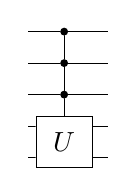
\begin{tikzpicture}
    \begin{yquant*}[loc/.style={style=blue, control style=blue}, nloc/.style={style=red, control style=red}]
    [drawing mode=quality]
    % registers
    qubit {} q0;
    qubit {} q1;
    qubit {} q2;
    qubit {} q3;
    qubit {} q4;
    % qubit {$\ket{\psi}$} psi;
    % [name=CCZ]
    % cnot q3, q1, q2,q4 | q0;
    box {$\ U\ $} (q3, q4) | q0, q1, q2;
    

    % \node[fit=(CCZ-0) (CCZ-1)] {CCZ};

    % h q0;
    % box {$R_2$} q0 | q1;
    % box {$R_3$} q0 | q2;
    % box {$R_4$} q0 | q3;

    % h q1;
    % box {$R_2$} q1 | q2;
    % box {$R_3$} q1 | q3;
    % h q2;
    % box {$R_2$} q2 | q3;
    % h q3;


    % swap (q0, q3) ;
    % swap (q1,q2);
    % box {$U^{2^0}$} psi | q3;
    % box {$U^{2^1}$} psi | q2;
    % box {$U^{2^2}$} psi | q1;
    % box {$U^{2^3}$} psi | q0;

    % barrier (q0, q1, q2, q3);
    
    hspace {1mm} -;

    % box {$QFT^\dagger$} (q0, q1, q2, q3);

    % hspace {2mm} -;
    % discard psi;


    % measure q0;
    % measure q1;
    % measure q2;
    % measure q3;

    % discard q0;
    % discard q1;
    % discard q2;
    % discard q3;
    % qubit {} eq[2]; % entangled qubits
    % [red]
    % init {$\rho_\Phi$} (eq);
    % qubit {$b$} b;
    % correlation: squigles
    % [nloc]
    % correlate (eq);
    
% $U_{\text{DCNOT}}[A,B; \Phi]$
    % [this subcircuit box style={draw, dashed, rounded corners,
    % fill=blue!0, inner ysep=5pt, "$U_{\tiny\textsc{DCNOT}}$" above},
    % register/default name=]
    % subcircuit {
    %     qubit {} a;
    %     qubit {} eq[2];
    %     qubit {} b;
        
    %     [loc] cnot eq[0]| a;
    %     [nloc]cnot eq[1]| eq[0];
    %     [loc] cnot b | eq[1];
    %     [loc] h eq[1];
    %     [nloc] z a | eq[1];
    % } (-);
    % % barrier (a,eq,b);
    % % [name=left] barrier (a,eq,b);
    % % operations
    
    % % barrier (a,eq,b);
    % % [name=right] barrier (a,eq,b);
    % output {Tr$_\Phi$} (eq);
    % % discard eq;
    % hspace {2mm} -;

    \end{yquant*}
%     \node[fit=(left-0) (left-3) (right-0) (right-3),
% draw, inner sep=6pt, "reversed c-\textsc{not}"] {};
\end{tikzpicture}

\end{document}

